 \documentclass[10pt,conference]{IEEEtran}
% \usepackage{epsfig}
\usepackage{graphicx}
% \usepackage{epstopdf}
% \usepackage{subfigure}
\usepackage{caption}
\usepackage{subcaption}
\usepackage{comment}
\usepackage{color} % for colored comments
\usepackage[normalem]{ulem} % strikethrough comment sout
\usepackage{url}
\usepackage{balance}
\usepackage{array}
\usepackage{tabulary}
\newcolumntype{M}[1]{>{\centering\arraybackslash}m{#1}}
\newcommand\MZ[1]{\textcolor{blue}{#1}}
\newcommand\DB[1]{\textcolor{magenta}{#1}}

\begin{document}

\title{Application-based QoS support with P4 and OpenFlow: A demonstration using Chameleon}

% \subtitle{[Extended Abstract]
% \titlenote{A full version of this paper is available as%\textit{Author's Guide to Preparing ACM SIG Proceedings Using
% \LaTeX$2_\epsilon$\ and BibTeX} at
% \texttt{www.acm.org/eaddress.htm}}}
%
% You need the command \numberofauthors to handle the 'placement
% and alignment' of the authors beneath the title.
%
% For aesthetic reasons, we recommend 'three authors at a time'

% i.e. three 'name/affiliation blocks' be placed beneath the title.
%
% NOTE: You are NOT restricted in how many 'rows' of
% "name/affiliations" may appear. We just ask that you restrict
% the number of 'columns' to three.
%
% Because of the available 'opening page real-estate'
% we ask you to refrain from putting more than six authors
% (two rows with three columns) beneath the article title.
% More than six makes the first-page appear very cluttered indeed.
%
% Use the \alignauthor commands to handle the names
% and affiliations for an 'aesthetic maximum' of six authors.
% Add names, affiliations, addresses for
% the seventh etc. author(s) as the argument for the
% \additionalauthors command.
% These 'additional authors' will be output/set for you
% without further effort on your part as the last section in
% the body of your article BEFORE References or any Appendices.

%\numberofauthors{1} %  in this sample file, there are a *total*
% of EIGHT authors. SIX appear on the 'first-page' (for formatting
% reasons) and the remaining two appear in the \additionalauthors section.
%
% You can go ahead and credit any number of authors here,
% e.g. one 'row of three' or two rows (consisting of one row of three
% and a second row of one, two or three).
%
% The command \alignauthor (no curly braces needed) should
% precede each author name, affiliation/snail-mail address and
% e-mail address. Additionally, tag each line of
% affiliation/address with \affaddr, and tag the
% e-mail address with \email.
%
% 1st. author
\author{
\IEEEauthorblockN{Divyashri Bhat\IEEEauthorrefmark{1}\IEEEauthorrefmark{2}, Jason Anderson\IEEEauthorrefmark{2}, Paul Ruth\IEEEauthorrefmark{3}, Michael Zink\IEEEauthorrefmark{1} and Kate Keahey\IEEEauthorrefmark{4}}\
      \IEEEauthorblockA{University of Massachusetts Amherst\IEEEauthorrefmark{1}, University of Chicago\IEEEauthorrefmark{2}, RENCI\IEEEauthorrefmark{3}, Argonne National Labs \IEEEauthorrefmark{4}}\
     \IEEEauthorrefmark{1}{dbhat,zink}@ecs.umass.edu, \IEEEauthorrefmark{2}jasonanderson@uchicago.edu, \IEEEauthorrefmark{3}pruth@renci.org, \IEEEauthorrefmark{4}keahey@mcs.anl.gov, 
}

% There's nothing stopping you putting the seventh, eighth, etc.
% author on the opening page (as the 'third row') but we ask,
% for aesthetic reasons that you place these 'additional authors'
% in the \additional authors block, viz.
% \additionalauthors{Additional authors: John Smith (The Th{\o}rv{\"a}ld Group,
% email: {\texttt{jsmith@affiliation.org}}) and Julius P.~Kumquat
% (The Kumquat Consortium, email: {\texttt{jpkumquat@consortium.net}}).}
% \date{30 July 1999}
% Just remember to make sure that the TOTAL number of authors
% is the number that will appear on the first page PLUS the
% number that will appear in the \additionalauthors section.

\maketitle
\begin{abstract}
Although SD-WANs are now widely deployed by several production networks, they are largely restricted to traffic engineering approaches based on layer 4 (L4) of the network protocol stack that result in improved Quality-of-Service (QoS) of the network overall without necessarily focussing on a specific application. However, the emergence of application protocols such as QUIC and HTTP/2 needs an investigation of layer 5-based (L5) approaches in order to improve users' Quality-of-Experience (QoE). In this demonstration, we leverage the capabilities of flexible switches that incorporate protocol-independent packet processing in order to intelligently route traffic based on application headers. We use Adaptive Bit Rate (ABR) video streaming as an example to show how such an approach can not only provide flexible traffic management but also improve application QoE. Our prototype consists of an actual deployment in a research testbed, Chameleon, and a state-of-the-art orchestration and visualization tool, Jupyter, that we integrate with Chameleon in order to provide a single vantage point for SDN experimenters.
\end{abstract}

% A category with the (minimum) three required fields
%\category{H.4}{Information Systems Applications}{Miscellaneous}
%A category including the fourth, optional field follows...
%\category{H.5.1}{Multimedia Information Systems}{Video}

%\terms{Measurement, Performance}

% \keywords{Software Defined Networks, OpenFlow, Applications, Software Defined Exchange, Performance} % NOT required for Proceedings

\section{Introduction}
\label{sec:intro}
While application protocols such as HTTP have evolved to provide reduced latency and efficient use of network resources \cite{rfc7540}, traffic engineering paradigms such as Software Defined Networking (SDN) have simultaneously emerged to provide better Quality-of-Service (QoS) through flexible routing and centralized network management. Several large-scale production Content Distribution Networks (CDNs) such as Google  \cite{Yap:2017}  %and Facebook \cite{Schlinker:2017} 
have implemented Software-Defined Wide Area Networks (SD-WANs) to efficiently perform application-aware routing at the peering edge. According to Cisco \cite{cisco-17}, downstream application traffic is predicted to account for 82\% of all Internet traffic by 2021. Moreover, the same report predicts that SD-WAN traffic will account for 25\% of all WAN traffic by 2021.

HTTP/2 incorporates several improvements over its predecessor, HTTP/1, which include a) multiplexing several streams into one TCP connection, b) server-push approaches, where content is delivered to a client without explicitly requesting it, and c) header compression for reduced latency. These improvements, particularly stream multiplexing, were devised to reduce page load time such that download requests for embedded objects such as images, video, etc., in a web page can be issued simultaneously (instead of sequentially). Similarly, the QUIC \cite{Langley:SIGCOMM:2017} protocol was introduced as a transport layer candidate for HTTP/2 with one basic difference: QUIC is based on UDP and can thus, be used to implement flexible congestion control as well. As protocols become more versatile to support high-bandwidth applications such as Adaptive Bit-Rate (ABR) video streaming and 360 Virtual Reality (VR), network architectures need to adapt in order to meet the demands of such applications worldwide. More recently, the introduction of flexible switch architectures such as \cite{Bosshart:2014} have paved the way for line-rate processing of application-layer headers \cite{jin2017netcache}.
Our demonstration investigates application-based QoS in centrally controlled networks. In particular, this work leverages the capability of protocol-independent packet processors (P4) \cite{Bosshart:2014} at the edge of the network to define a custom fixed-length application header and further, translate this into a Q-in-Q (802.1ad) tag \cite{IEEE802.1ad:standard} for the core network in order to perform QoS routing/provisioning.
%OpenFlow-based \cite{McKeown:2008}. 

In previous work \cite{acm-mmhttp2}, we demonstrated how HTTP/2-based multiplexing can be used to simultaneously fetch multiple qualities of video segments in order to improve the average bitrate quality and thereby, the Quality-of-Experience (QoE) of a client. In this demonstration, we show how HTTP/2 header information can be translated as a QoS requirement using P4-capable network elements to convert application layer header information into a Q-in-Q tag for differentiated routing via the core network using the Bring-Your-Own-Controller (BYOC) feature \cite{chameleon-byoc} provided by the Chameleon testbed \cite{Mambretti:2015}. Although we present a simple prototype using ABR streaming as an example, we believe the capabilities of such a system extend far beyond ABR segment retransmissions and can be used to implement systematic integration of Information Centric Networks (ICN) \cite{Ghodsi:2011} with legacy networks and simultaneous transmission of 360 video viewports \cite{hosseini2016adaptive}. %The remainder of this article provides a detailed description of our architecture (Sect. \ref{sec:design}), followed by our demonstration setup in Sect. \ref{sec:setup} and a Conclusion in Sect. \ref{sec:conclusion}.



\section{Design}
\label{sec:design}
\subsection{Application header-based Traffic Engineering}
\subsubsection{Q-in-Q}
\begin{comment}
\begin{figure}[htb!]
\includegraphics[width=1\columnwidth, trim={4cm 0cm 4cm 0cm}, angle=270,  scale=0.51] {figures/vlan_tag.pdf}
\caption{VLAN tag header insertion in Layer-2. 802.1Q was followed by 802.1ad in order to differentiate between customers on the same VLAN.}
\label{fig:vlan-tag}
\end{figure}
\end{comment}
%Figure \ref{fig:vlan-tag} 
%The IEEE 801.Q standard \cite{IEEE802.1Q:standard} describes the header frame format of the 802.1Q virtual LAN (VLAN) protocol, which was introduced in order to logically separate broadcast domains inside a Local Area Network (LAN). Following this, network service providers saw the need to similarly separate customers inside a VLAN and thus, a second 802.1Q tag was appended \cite{IEEE802.1ad:standard} to create Q-in-Q VLAN tunnels (802.1ad) that can easily be interpreted and altered by a network element with basic switching functionality. 
The IEEE 802.1ad standard \cite{IEEE802.1ad:standard} double-tagging was introduced to allow network service providers to separate traffic from different  VLANs as well as customers for better traffic management. Here, we use Q-in-Q tunneling to translate application-layer header information into link-layer headers at the edge before packets are forwarded to the core network. In particular, we focus on HTTP/2 application headers since they explicitly provide header fields that can be easily interpreted into Q-in-Q tags for better manageability.
\subsubsection{HTTP/2 Header}
\label{subsec:http2-header}
\begin{comment}
\begin{figure}[htb!]
%\centering
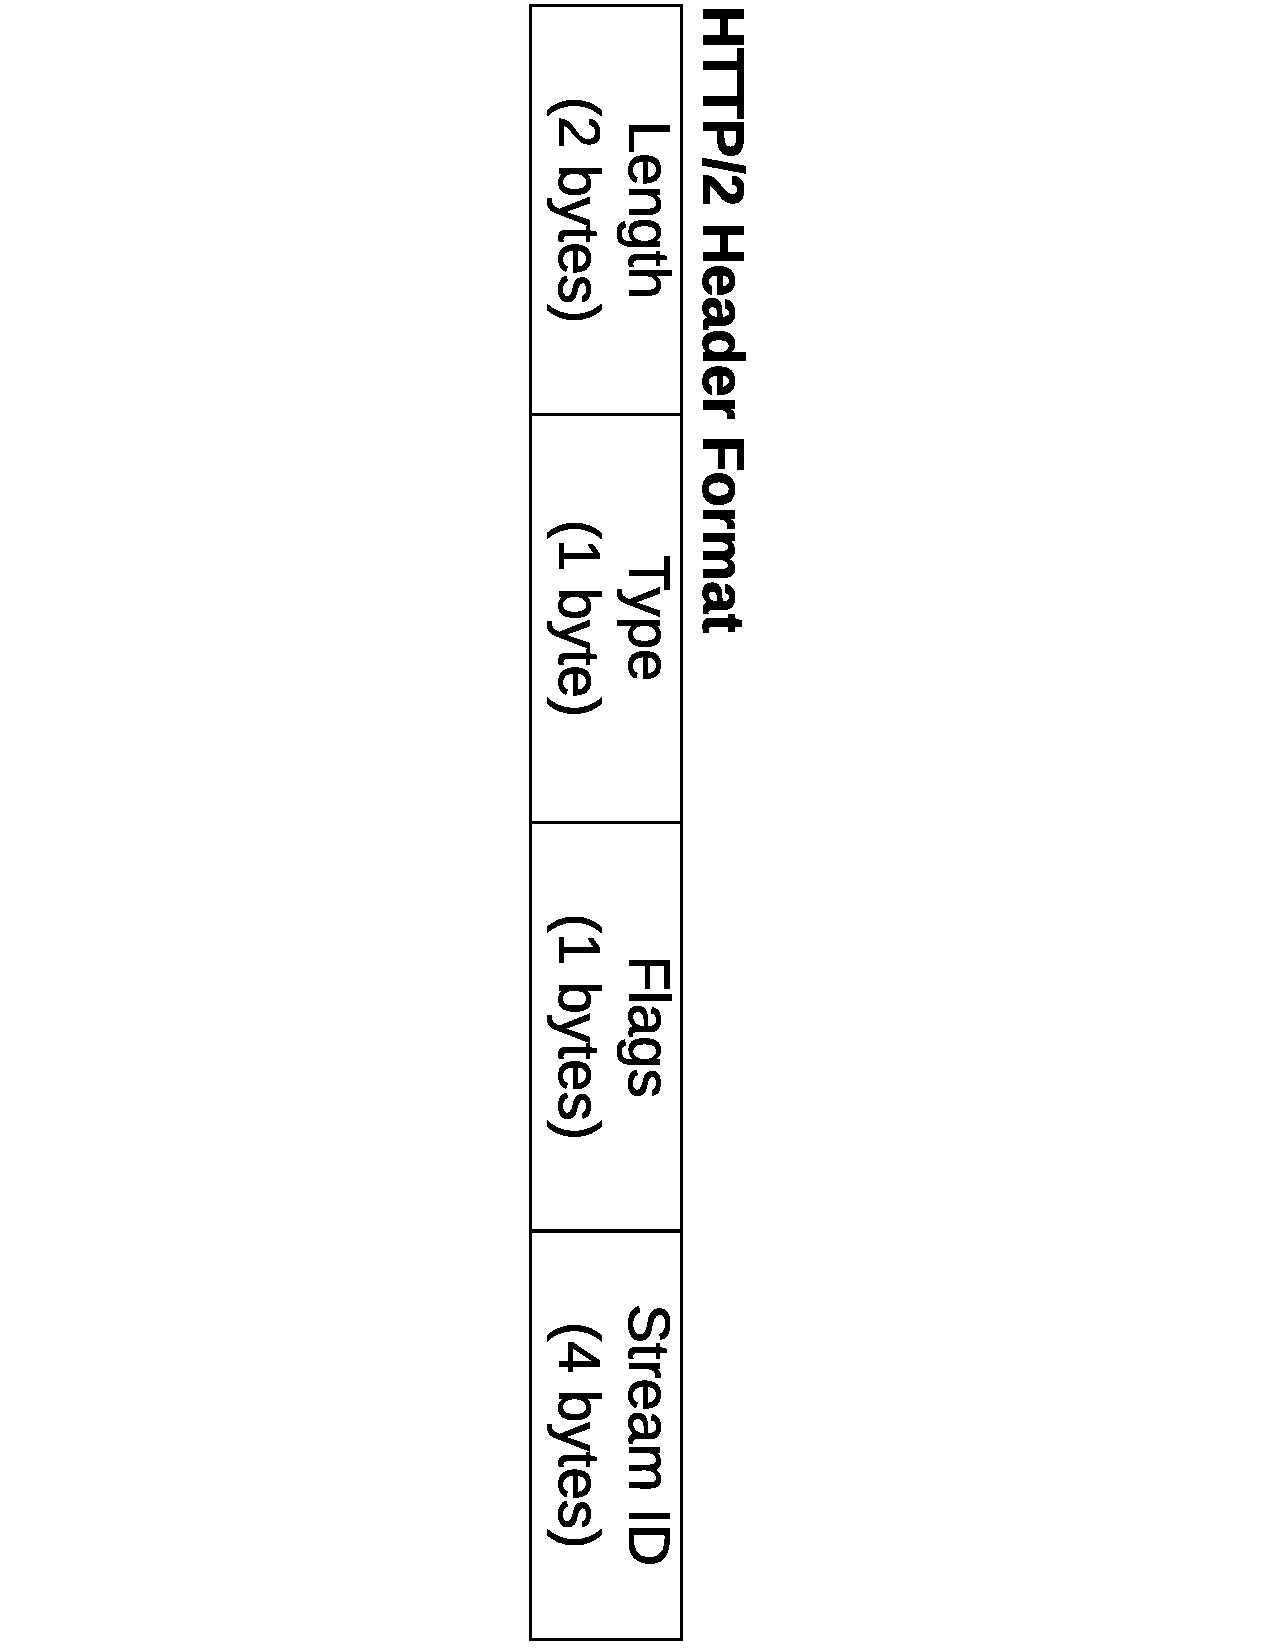
\includegraphics[width=1\columnwidth, trim={9cm 0cm 9cm 0cm}, angle=90, scale=0.13] {figures/HTTP2_header.pdf}
\caption{HTTP/2 Header Format: Common Eight-Byte Header}
\label{fig:http2-header}
\end{figure}
\end{comment}
As the number of objects embedded within a web page began to increase, the overhead due to variable length headers resulted in increased page load times for HTTP/1.1. Contrarily, HTTP/2 introduces a fixed length header and performs header compression in order to reduce perceived latency and increase goodput. It is interesting to note that HTTP/2 explicitly defines the \textit{Stream ID} field to multiplex several streams into a single TCP connection and thus, can be re-interpreted as a Q-in-Q tag by any link-layer device. %In general, the \textit{Stream ID} is used to differentiate between active concurrent downloads of embedded objects for a given web page.
In this work, we redefine the outer customer tag (C-TAG) as a \textit{Stream ID} tag using a flexible, protocol-independent packet processing language, P4 that can be programmed to interpret HTTP/2 headers. For the ABR video streaming application, \textit{Stream ID} is used to differentiate between two distinct bitrate qualities that are simultaneously downloaded by the client as described in our previous work \cite{acm-mmhttp2}. 
\subsection{System Architecture}
\begin{figure}
\vspace{-24pt}
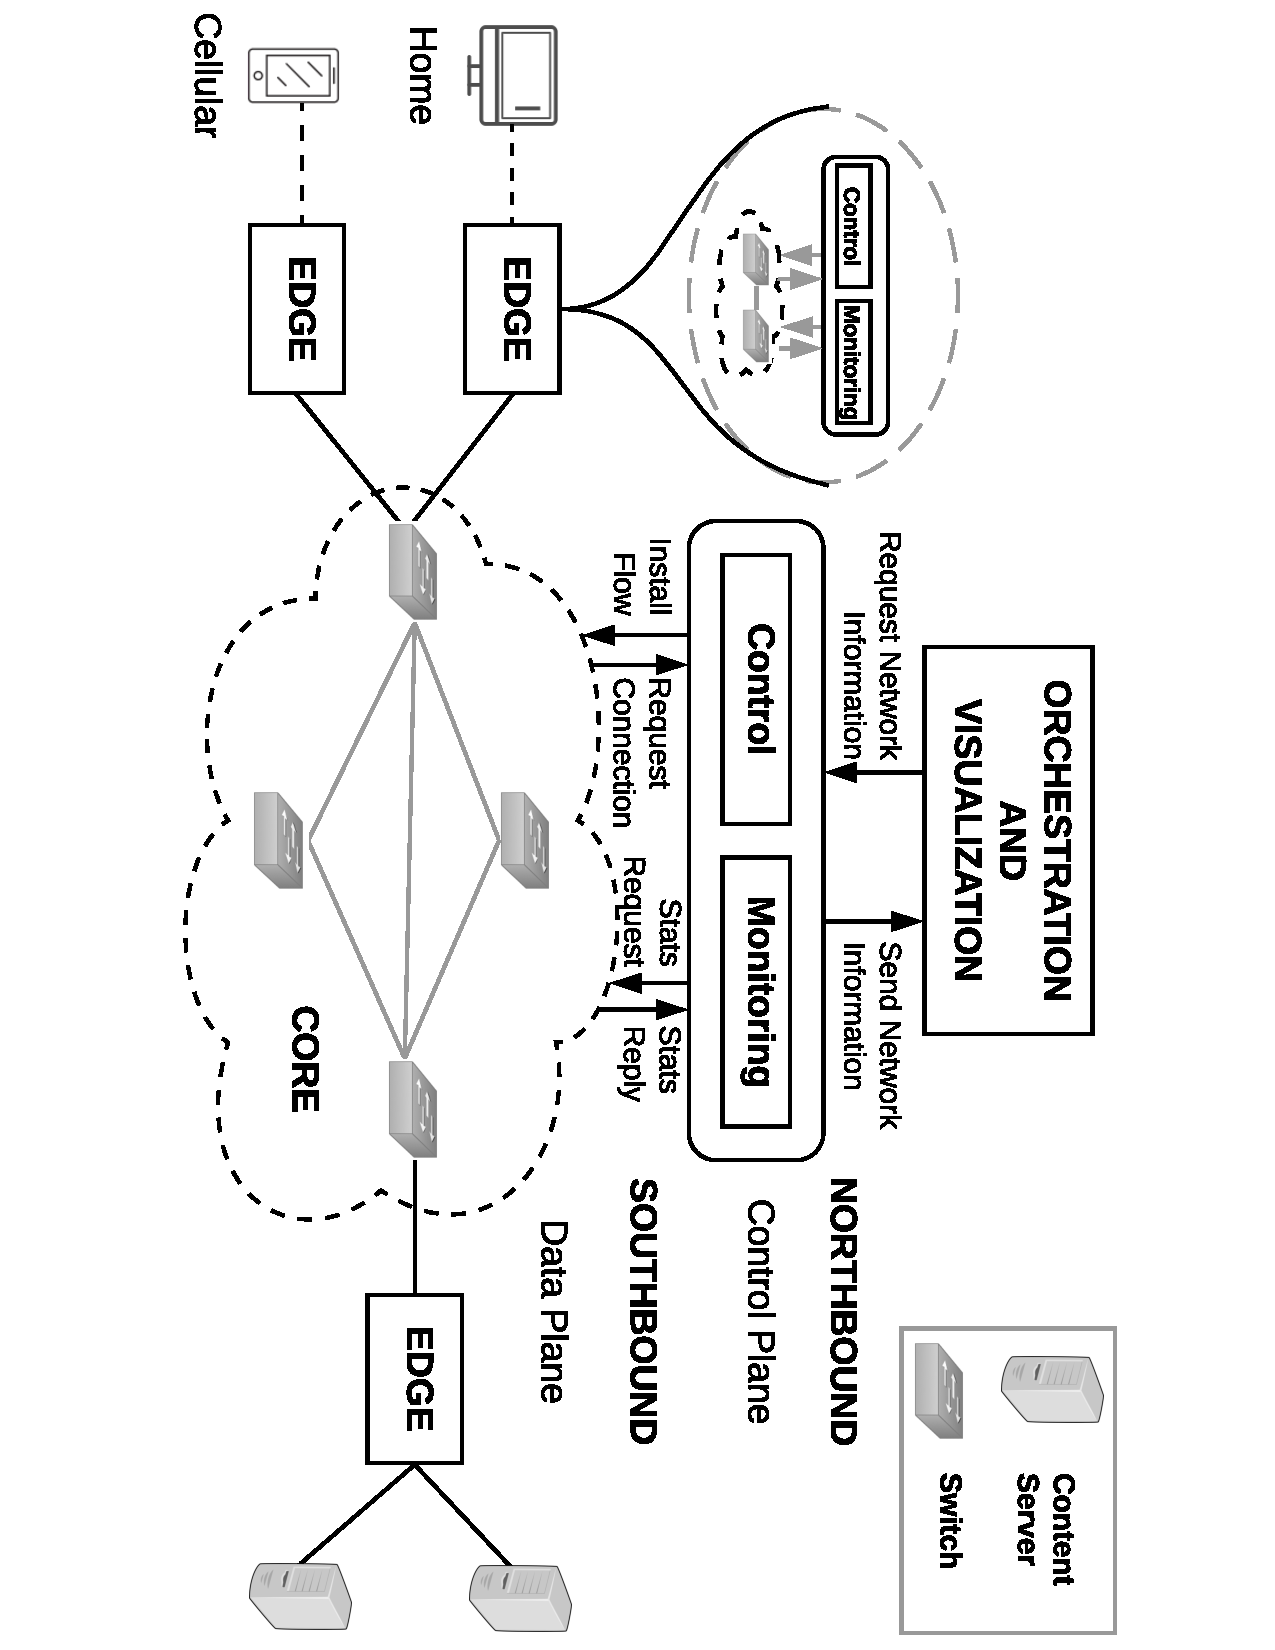
\includegraphics[ width=1\columnwidth, trim={2cm, 20cm, 0cm, 0cm}, angle=90, scale=0.7] {figures/NetworkArchitectureP4v2.pdf}
\caption{Architecture for QoE to QoS translation at the edge, which is envisioned as SD-WANs}
\label{fig:p4-of}
\vspace{-18pt}
\end{figure}
The main focus of our architecture is to translate application-layer header information into link-layer headers. We additionally includes a centralized component that allows network providers to orchestrate and visualize their network from a single interface.
Figure \ref{fig:p4-of} presents the architecture of our demonstration and consists of the following components:
\subsubsection{The Core}
For our architecture we assume a capability similar to that of a large-scale research testbed, ESNET\footnote{\url{https://www.es.net/network-r-and-d/experimental-network-testbeds/100g-sdn-testbed/}}, where the core or backbone network includes a programmable data-plane that performs fine-grained traffic engineering based on L2-L5 header information and is centrally controlled by an independent controller (denoted as \textit{Monitoring} and \textit{Control} in Fig. \ref{fig:p4-of}). However, we note that similar functionality can be incrementally deployed in production networks based on MPLS Traffic Engineering (MPLS-TE)\footnote{\url{https://www.cisco.com/c/en/us/products/collateral/ios-nx-os-software/multiprotocol-label-switching-traffic-engineering/}} techniques as well.
\subsubsection{The Edge}
Innovation at the edge such as SD-WANs \cite{Yap:2017} is driven by the tremendous growth in downstream application traffic and the advent of cloud computing. Here, the edge network also includes a programmable data-plane of several flexible switches that are centrally controlled by an independent controller. However, these switches can perform fine-grained traffic engineering using L5 header information as well. In order to peer with the core, the edge controller must translate information in L5 headers to L2-L4 headers before sending packets out into the core.
\subsubsection{Orchestration and Visualization}
Our system also includes a centralized component that aggregates monitoring information from the various controllers in order to provide a visual representation of network performance. 

The diagram also shows clients such as a wireless home network and cellular network that connect to an edge and receive requested content from a server located elsewhere on the edge network. The two edge networks are connected by the core. In the following section, we describe the setup for our demo including the platform and tools we use to run QoS translation experiments.



\section{Setup}
\label{sec:setup}
\begin{figure*}[htb!]
\centering
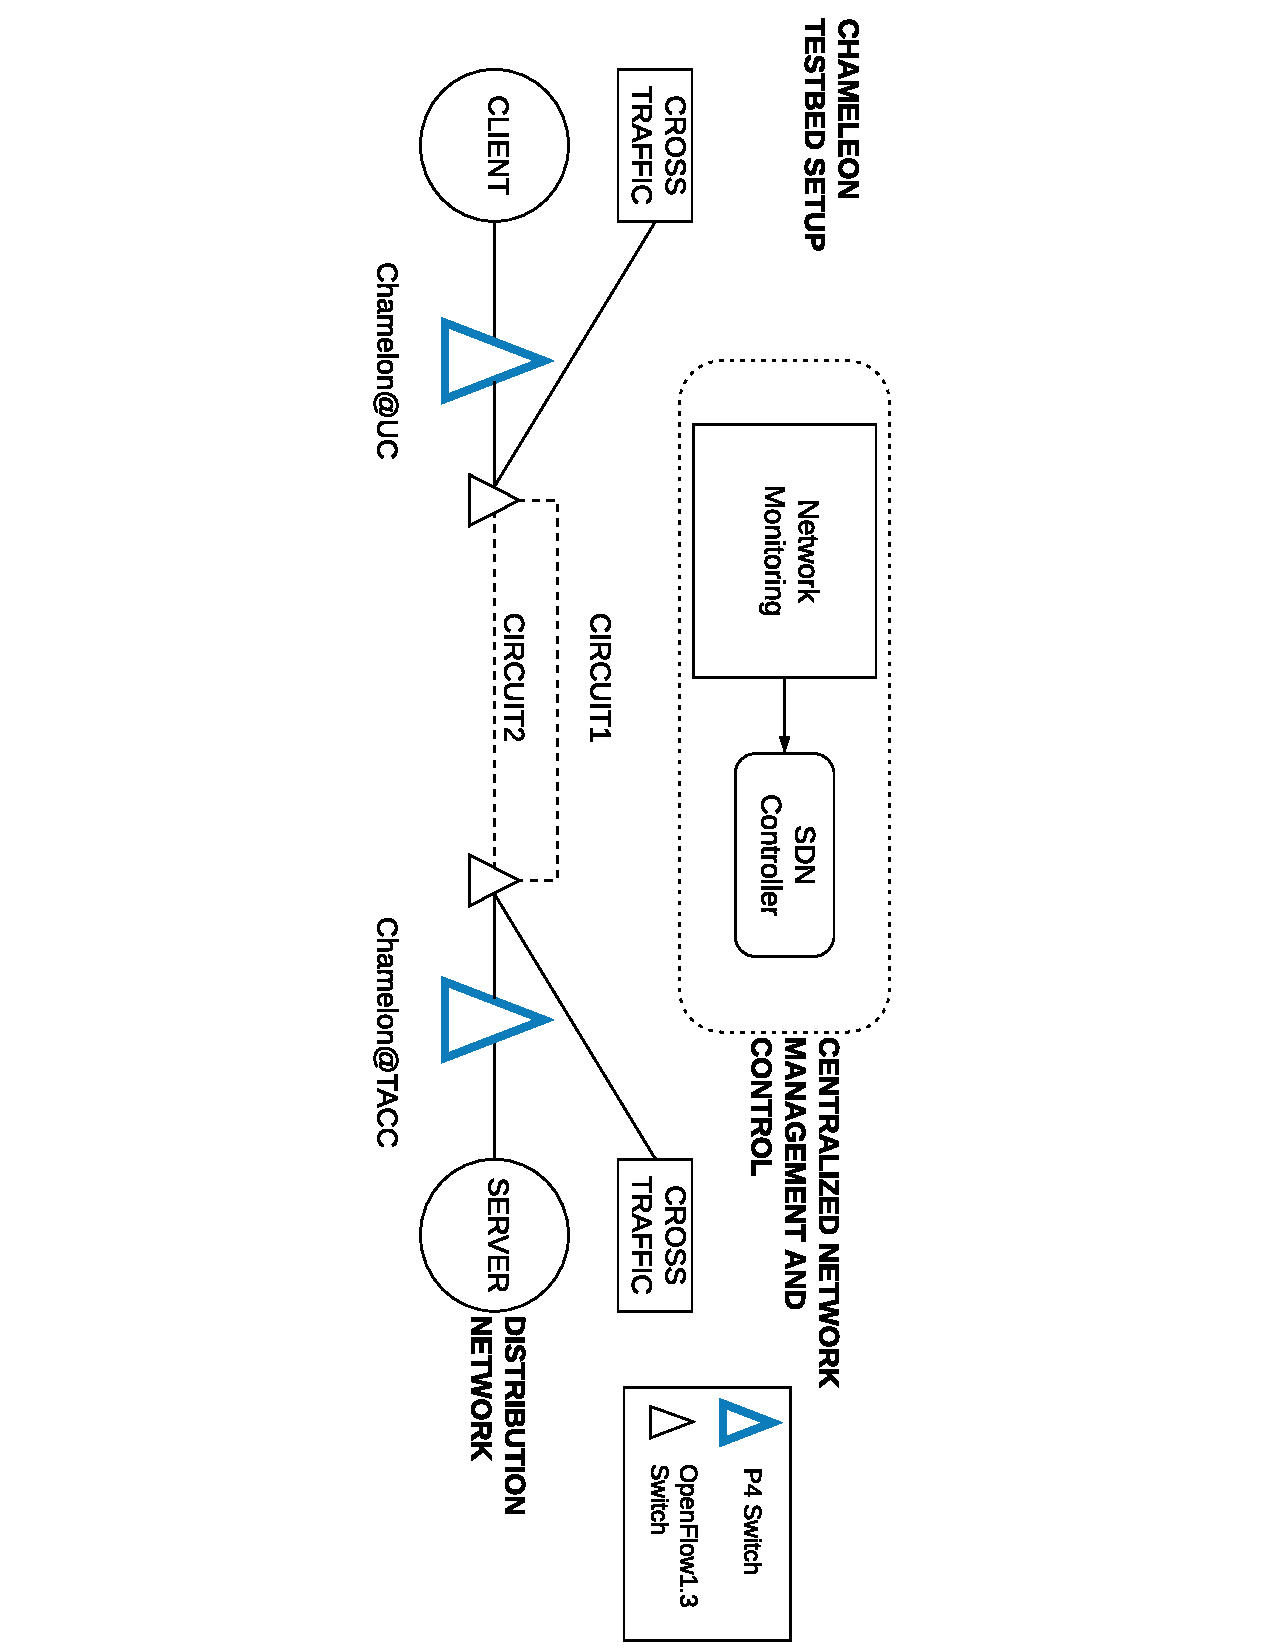
\includegraphics[width=.23\textwidth,trim={6cm 6cm 5cm 6cm}, angle=90] {figures/CHAMELEON_Exp.pdf}
\caption{Chameleon Testbed Setup: A HTTP/2 based video streaming client uses two disjoint paths to request multiple qualities of the same segment.}
\label{fig:p4-testbed}
\vspace{-14pt}
\end{figure*}
\subsection{Chameleon Testbed}
The Chameleon testbed is a deeply reconfigurable testbed that is suitable for large-scale prototyping of distributed systems and software defined networks. In this work, we leverage the recently released Bring-Your-Own-Controller feature along with previously existing capabilities of the Chameleon Cloud to create a prototype of our architecture. Figure \ref{fig:p4-testbed} shows the setup of our testbed, which we describe in detail.
\subsubsection{HTTP/2 application}
For the HTTP/2 application we instantiate two bare-metal nodes: one that emulates a Web server using the open source \texttt{Caddy} (version=0.10.10) software and another that emulates an ABR video streaming client, \texttt{AStream}{\footnote{\url{https://github.com/pari685/AStream}}}, that we modify to use an open-source Python-based library, \texttt{hyper}\footnote{\url{https://github.com/Lukasa/hyper}}, that downloads video content using HTTP/2. Note that the cross traffic nodes are bare-metal machines used to create various network congestion scenarios using \texttt{Iperf3}\footnote{\url{https://iperf.fr/iperf-download.php}} for controlled experiments.
\subsubsection{P4 Switch\cite{Bosshart:2014}}
We install the behavioral model, \texttt{BMV2}\footnote{\url{https://github.com/p4lang/behavioral-model}}, software switch components in a bare-metal node, which emulates a P4-capable switch, and then use the \texttt{P4Runtime}\footnote{\url{https://github.com/p4lang/PI}} tool to programmatically install rules into each switch. In future, we plan to replace this with a hardware ASIC P4 switch\footnote{\url{https://www.barefootnetworks.com/products/brief-tofino/}} that has only recently become available. 
\subsubsection{OpenFlow Switch}
OpenFlow \cite{McKeown:2008}, a widely-used implementation of SDN, is available to experimenters as a Virtual Forwarding Context (VFC), a functionality provided by Corsa switches, which enables each testbed user to provision a nearly-isolated instance of an OpenFlow (v1.3) switch. After HTTP/2 headers are translated into Q-in-Q tags as described in Sect. \ref{subsec:http2-header}, the application packets are forwarded through the Corsa switch into the core network.
\subsubsection{Core Network}
In this demonstration, we provision two VLAN circuits (denoted as \textit{Circuit1} and \textit{Circuit2}) between University of Chicago (UC) and Texas Advanced Computing Center (TACC) using the Advanced Layer-2 Service (AL2S) implemented by Internet2, which is a network service provider for collaborative research\footnote{\url{https://www.internet2.edu/products-services/advanced-networking/layer-2-services/#features-al2s}}.
\subsubsection{Centralized Management and Control}
For orchestration and visualization, we use Jupyter Notebooks \cite{kluyver2016jupyter}, an open-source web tool particularly suited for reproducible experiments. For this demonstration, Jupyter runs inside Chameleon and provides us with a single interface not only to run the controller and the ABR video streaming application but also to visualize network traffic and QoE metrics. 
 %We will provide a laptop that connects to the monitor and allows conference attendees to view as well as use the Jupyter web instance to interact with our experiment. 




\section{Demo}
\label{sec:demo}
We will use the testbed setup described above to systematically compare QoE metrics such as average quality bitrate for two traffic engineering approaches: one where ABR video streaming retransmissions are differentially routed using a flexible switch and another where retransmissions are classified as regular HTTP traffic without any preferential treatment. Since all of the experiment components are located in a public cloud, for this demonstration we will require a large monitor with a HDMI connector  to allow conference attendees to view as well as use the Jupyter web instance to interact with our experiment and two power outlets.


\section{Conclusion}
\label{sec:conclusion}
In this work, we show how flexible switches at the edge can be used to translate application layer header information into link layer headers to differentially route distinct qualities of ABR video segments in order to improve QoE of a HTTP/2-based application. Our demonstration is performed in a geographically distributed testbed, Chameleon, using open source orchestration and visualization tools that are easily available to researchers. 

\input{Acknowledgements}

%
% The following two commands are all you need in the
% initial runs of your .tex file to
% produce the bibliography for the citations in your paper.
\bibliographystyle{IEEEtran}
\balance
\bibliography{paper}  % sigproc.bib is the name of the Bibliography in this case
% You must have a proper ".bib" file
%  and remember to run:
% latex bibtex latex latex
% to resolve all references
%
%\bibliographystyle{IEEEtran}
%\balance\bibliography{paper}  
\end{document}
